\subsection{Proposed architecture hpcasia}

\begin{figure}
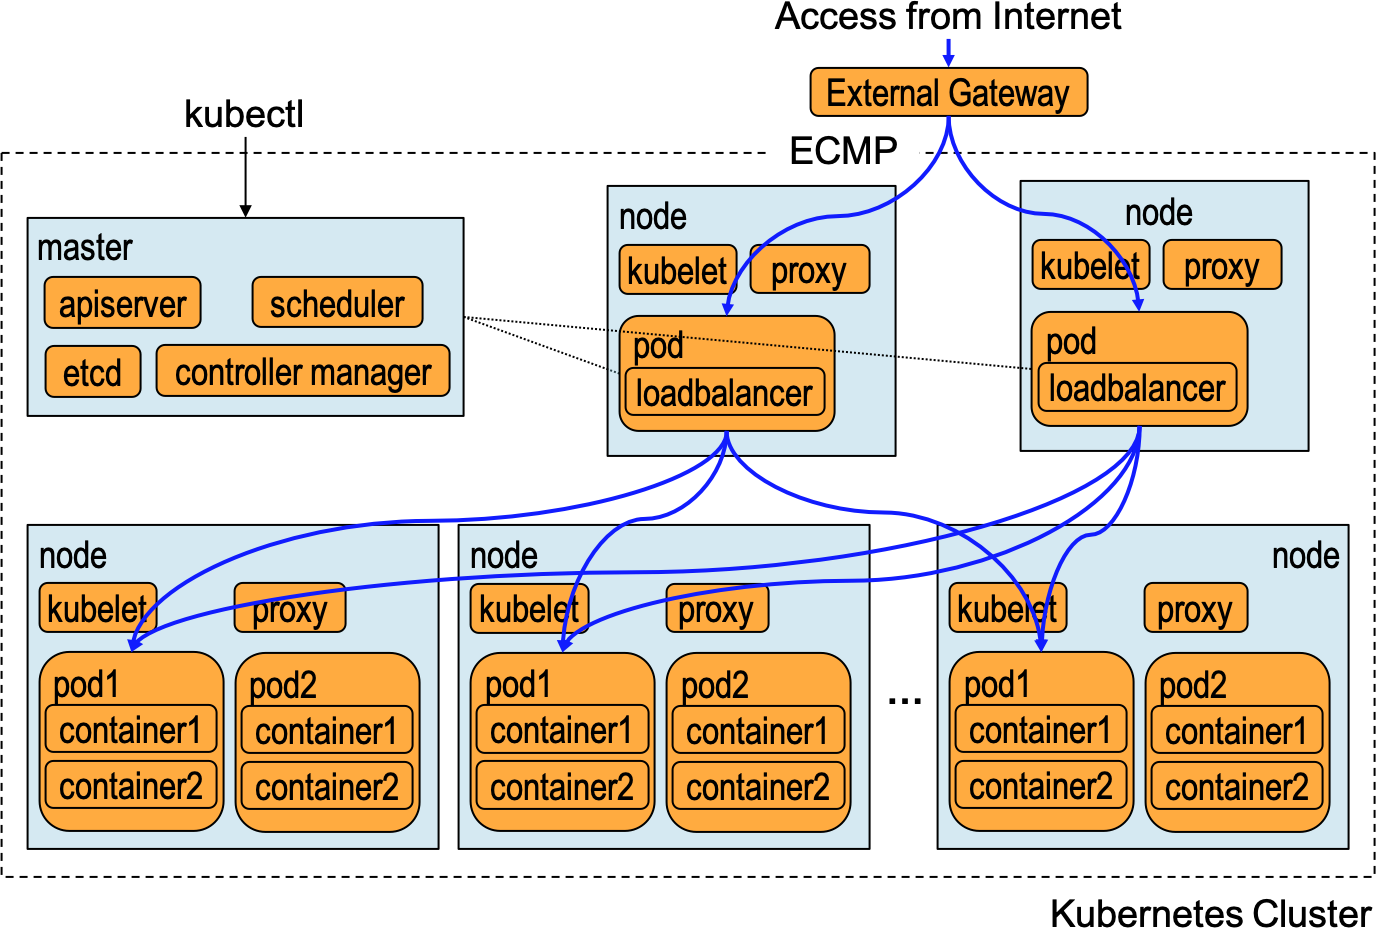
\includegraphics[width=\columnwidth]{Figs/K8sProposed}
\caption{Kubernetes cluster with proposed load balancer.}
\label{fig:K8sProposed}
\end{figure}

Figure~\ref{fig:K8sProposed} shows the proposed  Kubernetes cluster architecture, 
which has the following characteristics:
1) Each load balancer itself is run as a {\em pod} by Kubernetes. 
2) Load balancer configurations are dynamically updated based on information about running {\em pods}.
%%3) There exist multiple load balancers for redundancy. 
The proposed load balancer can resolve the conventional architecture problems, as follows:
Since the load balancer itself is containerized, load balancer can run in any environment including on-premise data centers, 
even without external load balancers that is supported by Kubernetes.
The incoming traffic is directly distributed to designated {\em pods} by the load balancer. 
It makes the administration, e.g. finding malfunctions, easier.

We designed the proposed load balancer using three components, IPVS, keepalived, and a controller. 
These components are placed in a Docker container image.
The IPVS is a Layer-4 load balancer capability, which is included in the Linux kernel 2.6.0 released in 2003 or later, 
to distribute incoming Transmission Control Protocol(TCP) traffic to 
{\em real servers}\footnote{The term, {\em real servers} refers to worker servers that will respond to incoming traffic, 
in the original literature\cite{Zhang2000}. We will also use this term in the similar way.}\cite{Zhang2000}. 
For example, IPVS distributes incoming Hypertext Transfer Protocol(HTTP) traffic destined for a single destination IP address, 
to multiple HTTP servers(e.g. Apache HTTP or nginx) running on multiple nodes in order to improve the performance of web services.
Keepalived is a management program that performs health checking for {\em real servers}
and manage IPVS balancing rules in the kernel accordingly.
It is often used together with IPVS to facilitate ease of use.
Although keepalived also supports Virtual Router Redundancy Protocol(VRRP)\cite{hinden2004virtual}, the authors leave that topic for future work.
The controller is a daemon that periodically monitors the {\em pod} information on the master, 
and performs various actions when such information changes.
Kubernetes provides ingress controller framework as the Go Language(Golang) package to implement such controllers. 
We have implemented a controller program that will feed {\em pod} state changes to keepalived 
using this framework. 

These are the main ideas behind our proposal. In the following section, we will explain their implementation in detail.
